\FloatBarrier

\begin{figure}[h!]
	\centering
	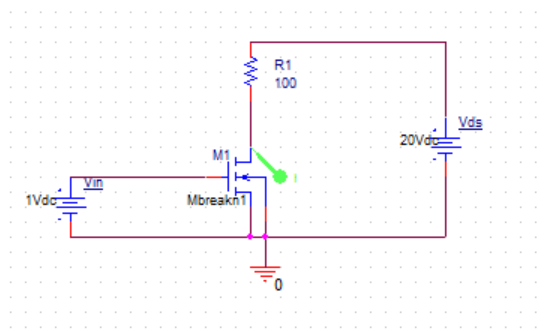
\includegraphics[scale=1]{./images/circuit1.PNG}
	\caption{Common Source Amplifier with Passive Load}
	\label{fig:circuit1}
\end{figure}

\FloatBarrier

\FloatBarrier

\begin{figure}[h!]
	\centering
	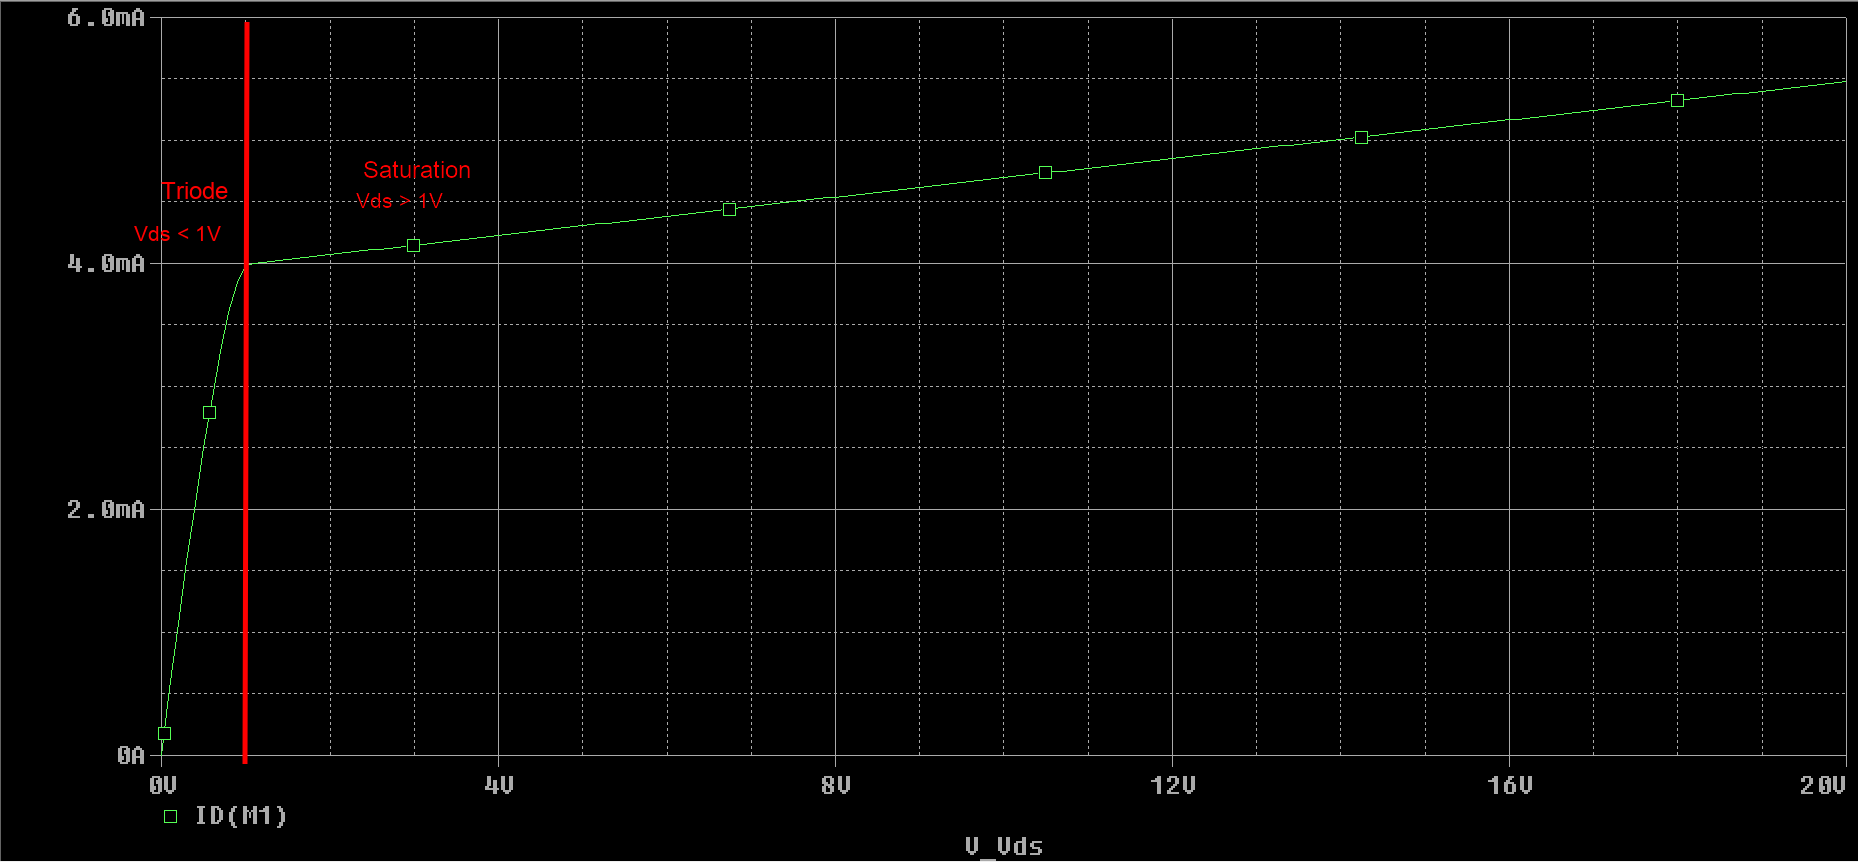
\includegraphics[scale=0.25]{./images/id_vs_vds.PNG}
	\caption{$i_D$ versus $V_{DS}$}
	\label{fig:id_vs_vds}
\end{figure}

\FloatBarrier

The curve in figure (\ref{fig:id_vs_vds}) is the expected $i_D$ versus $V_{DS}$ curve of an NMOS transistor with channel length modulation effects. From the diagram, $V_{GS} - V_T$ appears to be $1$\si{\volt} since that is where the edge between triode and saturation occurs. \uline{The transistor operates in triode for $V_{DS} < V_{GS} - V_T = 1$\si{\volt}, and it operates in saturation for $V_{DS} > 1$\si{\volt}.}

\FloatBarrier

\begin{figure}[h!]
	\centering
	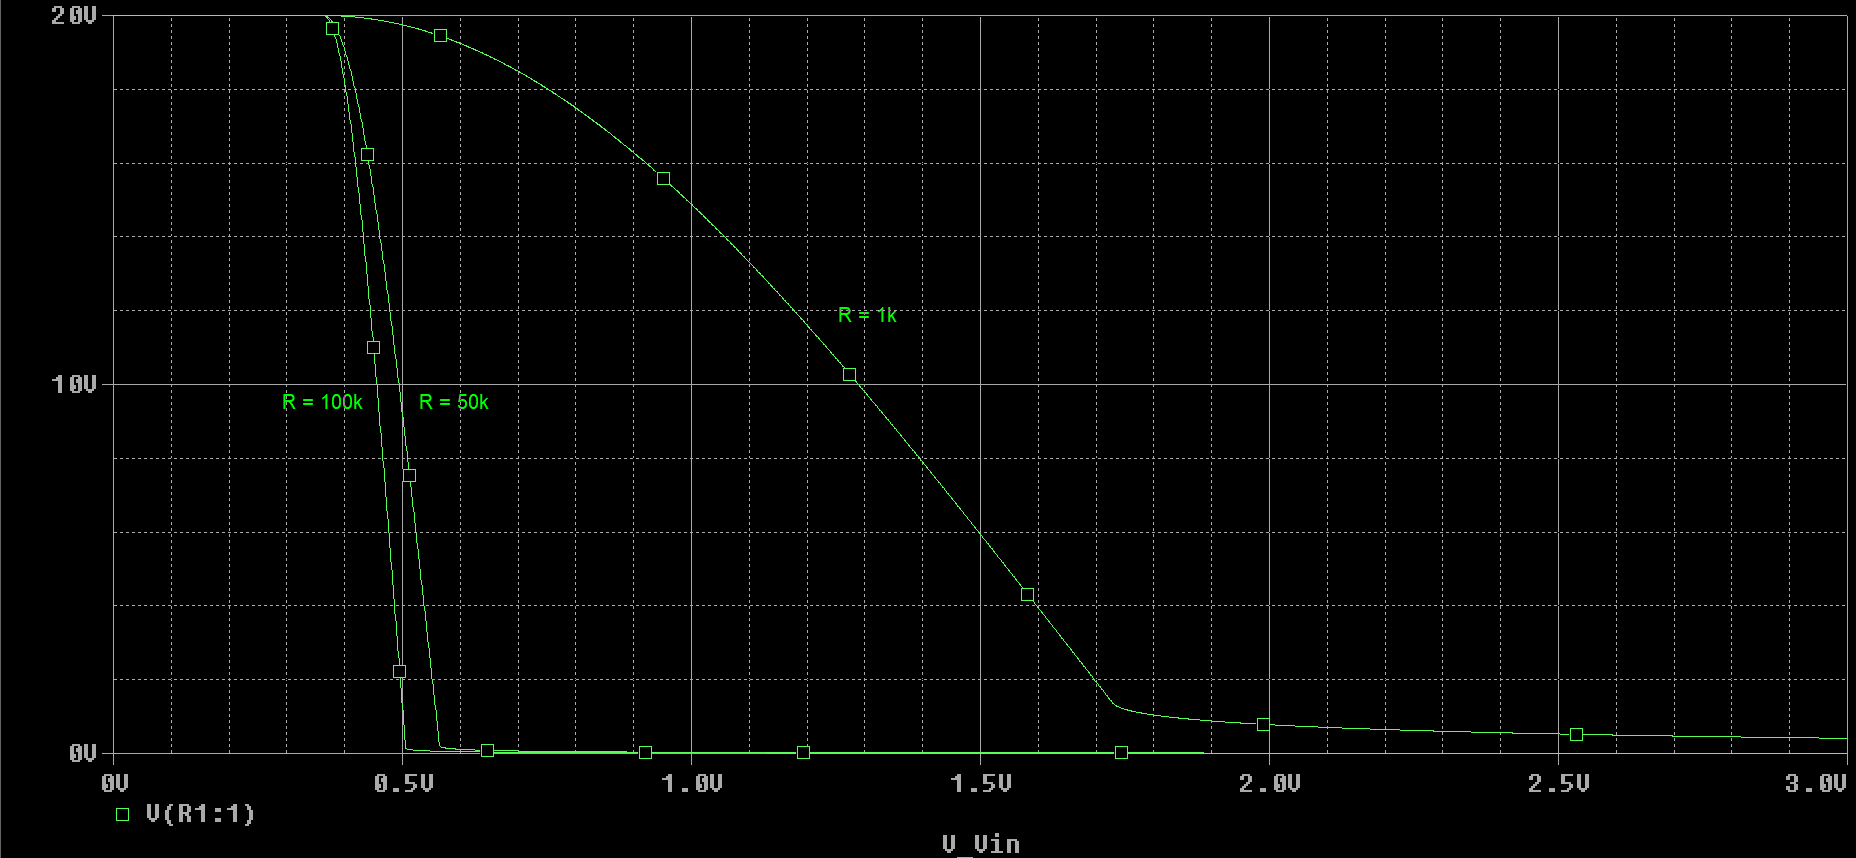
\includegraphics[scale=0.50]{./images/vout_vs_vin.PNG}
	\caption{Voltage Transfer Characteristic}
	\label{fig:vout_vs_vin}
\end{figure}

\FloatBarrier

For low values of $V_{in}$, the transistor remains in cutoff. As a result, no voltage drops over the resistor since no current flows. Therefore, $V_{DS} = V_{out}$ is maximized at the supply voltage. As $V_{in}$ is increased, the conductive channel forms and current can flow. However, assuming the current is a continuous function of $V_{in}$, it starts off at relatively small values, meaning that the voltage drop over the resistor is still small. Thus, the transistor's $V_{DS}$ is still large and far exceeds $V_{in}$. As $V_{in}$ increases, more current can flow, the resistor eats up more of the supply voltage, and $V_{out}$ rapidly drops. For sufficiently large values of $V_{in}$, the transistor enters the triode region since $V_{DS}$ becomes comparable in magnitude to $V_{in}$. At this point, the current no longer follows a linear relationship with $V_{in}^2$ and instead begins following a linear relationship with $V_{in}$. As a result, the resistor's voltage does not increase as rapidly and $V_{out}$ therefore does not decrease as rapidly as they do in the saturation region. \\

Certain applications may call for other properties, but the common source amplifier should act as an inverter or a voltage amplifier. As an inverter, the steepest drop from the supply voltage to ground is desired to prevent undefined behavior between a "0" and a "1". This occurs when $R = 100$\si{\kilo\ohm}. As a voltage amplifier, high linearity is desired. The linearity of the $R = 100$\si{\kilo\ohm} and $R = 50$\si{\kilo\ohm} curves are nearly the same and better than the $R = 1$\si{\kilo\ohm} curve. \\

Furthermore, a steeper slope of the curve is typically better. For more gradual slopes, the AC signal needs to vary a bit more to achieve the same output voltage. The closer the AC signal's magnitude comes to the overdrive voltage $V_{ov}$, the more distortion occurs in the output waveform. So, the preserve the input signal's shape at the output, a steeper slope is required. \uline{So, overall, the best choice of resistor value is $R = 100$\si{\kilo\ohm}.} \\

When the common source amplifier is used for its voltage amplification characteristics, a bias current is typically used to tune the amplifier accordingly. \uline{The amplifier should operate near the middle of the saturation region.} Linearity is achieved in the saturation region, whereas cutoff and triode give rise to nonlinearities in the output signal such as waveform clamping. Furthermore, the transistor gets the maximum signal swing at the middle of the saturation region, letting it operate over a wider range of input signal amplitudes. However, increasing $V_{GS}$ can increase the amplifier's gain, as is discussed below, but leads to a lower output swing. So, whenever gain is preferred over output swing, the voltage can be increased beyond the bias point in the middle of the saturation region. \\
